\section{Proposta}

Este trabalho tem como proposta a utilização de um modelo de inteligência artificial para segmentação panóptica que irá classificar os pixeis na imagem e permitir que os usuários gerem mapas procedurais a partir da seleção de um dos segmentos da imagem.

Utilizando o modelo EfficientPS é possível fazer a segmentação panóptica, segue exemplos nas \crefrange{fig:segmantations_1}{fig:segmantations_2}. O modelo citado está disponível no GitHub dos próprios autores \citeonline{mohan2020efficientps}.
% e será treinado com a combinação de pelo menos dois conjuntos de dados citados anteriormente.
No resultado apenas será identificado os pixeis de classes contidas nos conjuntos de dados escolhidos, portanto é possível que em uma imagem não seja identificado nada:

\begin{figure}[!ht]
	\centering
    \caption{Imagem de entrada para rede neural.}
	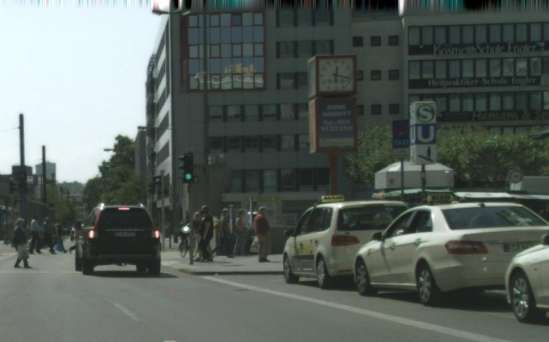
\includegraphics[width=0.6\textwidth]{figures/segmantations_1.png}
    \legend{Fonte: \citeonline{kirillov2019panoptic}}
	\label{fig:segmantations_1}
\end{figure}

\begin{figure}[!ht]
	\centering
    \caption{Imagem saída de um modelo de segmentação panóptica.}
	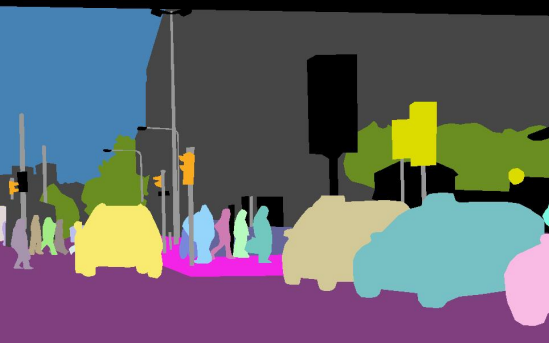
\includegraphics[width=0.6\textwidth]{figures/segmantations_2.png}
    \legend{Fonte: \citeonline{kirillov2019panoptic}}
	\label{fig:segmantations_2}
\end{figure}

Após a segmentação da imagem — como ilustra a \cref{fig:segmantations_2} — o usuário poderá selecionar uma das áreas coloridas da imagem que será utilizada para gerar a ilha.

Em seguida será criado um diagrama de Voronoi (pode ser observado na \cref{fig:diagrama_voronoi}), esse diagrama será utilizado para marcar a localização da ilha, assim gerando o mapa e os biomas a partir da atribuição de propriedades para cada ponto, polígono e reta do diagrama.

O resultado esperado pode ser contemplado na \cref{fig:resultado_geracao}, onde o azul representa o oceano, o verde retrata a floresta e o cinza caracteriza uma montanha.

\begin{figure}[!ht]
	\centering
    \caption{Ilha gerada a partir da segmentação panóptica e aplicando um filtro com o diagrama de Voronoi, azul representa oceano, verde floresta, cinza montanhas.}
	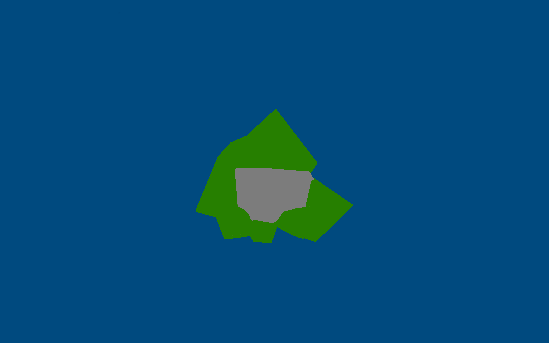
\includegraphics[width=0.6\textwidth]{figures/segmantations_pnl.png}
    \legend{Fonte: Criação própria}
	\label{fig:resultado_geracao}
\end{figure}

